\chapter{Dualidad de Fourier, momento y movimiento de una partícula libre}

\section{De los fundamentos a los ejemplos}

El entrelazamiento ocupa un lugar central en la mecánica cuántica, pero ya hemos expuesto suficientemente sus fundamentos como para empezar a aplicarlos. Hasta ahora, el curso se ha apoyado deliberadamente en sistemas pequeños: un espín, un aparato giratorio, una lista finita de resultados y mediciones repetidas a partir de las cuales se infieren probabilidades. Estos experimentos son lógicamente más sencillos que el recorrido histórico que condujo al descubrimiento de la mecánica cuántica, pero contienen los ingredientes operacionales mínimos.

\begin{classroomqa}\audiencequestion{¿Qué desempeña en la mecánica cuántica el papel del reducido conjunto de puntos de partida empíricos de Newton?}\lecturerresponse{Un modelo mínimo es el aparato giratorio de espín. Se prepara un espín, se elige un eje, se acciona el control de medición, se registra \(+1\) o \(-1\) y se repite el experimento hasta conocer las frecuencias de los resultados. El espacio vectorial, los observables, las amplitudes y la regla de Born organizan esas estadísticas. Históricamente, la teoría surgió de un conjunto mucho más rico de fenómenos atómicos, pero, desde el punto de vista lógico, este experimento de dos resultados basta para poner de manifiesto su estructura.}\end{classroomqa}

\begin{classroomqa}\audiencequestion{¿Hay que llevar a cabo el mismo procedimiento estadístico para cada magnitud física, como el espín o el momento?}\lecturerresponse{Sí. Un observable está asociado a una clase de montajes experimentales y a sus posibles resultados. El formalismo predice la distribución una vez especificados el estado y el observable, pero el significado físico del observable se fundamenta en cómo se mide.}\end{classroomqa}

Antes de dejar atrás el entrelazamiento, merece una respuesta completa una pregunta de la discusión anterior. Consideremos dos electrones con sectores singlete y triplete, e incluyamos el campo de radiación como otro subsistema cuántico. El campo de radiación tiene un estado de vacío \(\ket{0_\gamma}\) y un estado de un fotón \(\ket{1_\gamma}\). El propio número de partículas puede estar en superposición; no hay ninguna regla que limite la superposición a estados con un número fijo de partículas.

Para la transición idealizada que comentamos en clase, el estado inicial de los electrones, sin entrelazamiento, puede escribirse como una superposición de componentes singlete y triplete:
\begin{equation}
\ket{\uparrow\downarrow}
=
\frac{1}{\sqrt{2}}
\left(\ket{S}+\ket{T_0}\right).
\end{equation}
Como inicialmente no hay ningún fotón, el estado es
\begin{equation}
\ket{\Psi(0)}
=
\frac{1}{\sqrt{2}}
\left(\ket{S}+\ket{T_0}\right)
\otimes\ket{0_\gamma}.
\label{eq:l9-initial-radiative-state}
\end{equation}
La componente singlete permanece en un estado singlete sin emisión, mientras que la componente triplete excitada puede relajarse al singlete y emitir un fotón:
\begin{align}
\ket{S}\ket{0_\gamma}
&\longrightarrow
\ket{S}\ket{0_\gamma}, \\
\ket{T_0}\ket{0_\gamma}
&\longrightarrow
\ket{S}\ket{1_\gamma}.
\end{align}
Por linealidad, se obtiene
\begin{equation}
\ket{\Psi_{\mathrm{final}}}
=
\ket{S}\otimes
\frac{\ket{0_\gamma}+\ket{1_\gamma}}{\sqrt{2}}.
\label{eq:l9-final-radiative-state}
\end{equation}

\begin{figure}[htbp]\centering
\includegraphics[width=0.88\textwidth]{lecture_09_figure_01.png}\caption{El estado de los electrones se descompone en componentes singlete y triplete, y se toma el producto tensorial de estas con el vacío del campo de radiación antes de la relajación radiativa.}\lectureframe{00:05:10}\end{figure}

La expresión final es un producto entre el par de electrones y el campo de radiación. Los dos electrones están entrelazados entre sí porque \(\ket{S}\) está entrelazado, mientras que el campo de radiación queda en una superposición de cero y un fotón. Este ejemplo es sutil porque la interacción ha redistribuido el entrelazamiento: el estado inicial de los electrones, que era un producto, evoluciona a un par de electrones entrelazado; sin embargo, el estado final idealizado de electrones y radiación se factoriza.

\begin{classroomqa}\audiencequestion{¿Podría cualquier fotón incidente invertir la transición y desentrelazar los electrones?}\lecturerresponse{No. El proceso inverso en el tiempo requiere el estado de fotón, el modo, la fase, la energía y la historia de interacción adecuados. Reflejar el fotón emitido para que regresara era una manera abreviada de describir cómo disponer la evolución inversa del sistema cerrado completo; no implicaba que cualquier fotón fuera a deshacer el entrelazamiento.}\end{classroomqa}

\begin{classroomqa}\audiencequestion{¿Qué hace que el triplete emita si no se ha introducido ningún campo magnético externo?}\lecturerresponse{Los electrones interactúan entre sí y con el campo electromagnético cuantizado. Su interacción dependiente del espín hace que una configuración de espín tenga menor energía, y el exceso de energía puede salir en forma de radiación. No hace falta ningún aparato de medición externo: se trata de la dinámica unitaria habitual del sistema compuesto por los electrones y el campo.}\end{classroomqa}

Aclarado este último punto, dejamos ahora de lado el espín y estudiamos el problema de movimiento más sencillo: una partícula en una recta unidimensional.

\section{Ondas planas y el par de Fourier}

Antes de volver a la física, necesitamos una digresión matemática. Empecemos con
\begin{equation}
e^{ipx}=\cos(px)+i\sin(px).
\end{equation}
En este punto, \(p\) es simplemente un número real que determina la rapidez de la oscilación. La expresión no depende del tiempo, así que todavía no describe una onda en movimiento. Se llama onda plana porque, como función de \(x\), tiene la forma sinusoidal habitual.

Una amplia clase de funciones suficientemente regulares puede descomponerse en estos modos. Nos limitaremos a funciones que se comporten lo bastante bien para que las integrales siguientes estén definidas: no pueden divergir en el infinito espacial, y más adelante las funciones de onda físicas serán de cuadrado integrable. Con una convención de normalización simétrica, el par de Fourier es
\begin{align}
\psi(x)
&=
\int_{-\infty}^{\infty}
\frac{dp}{\sqrt{2\pi}}\,
\widetilde{\psi}(p)e^{ipx},
\label{eq:l9-fourier-forward}\\
\widetilde{\psi}(p)
&=
\int_{-\infty}^{\infty}
\frac{dx}{\sqrt{2\pi}}\,
\psi(x)e^{-ipx}.
\label{eq:l9-fourier-inverse}
\end{align}
El coeficiente \(\widetilde{\psi}(p)\) es la amplitud compleja del modo con etiqueta de Fourier \(p\). Los factores \(1/\sqrt{2\pi}\) son convencionales; poner uno en cada sentido hace que las dos fórmulas parezcan recíprocas. El signo relativo menos en el exponente es esencial.

\begin{figure}[htbp]\centering
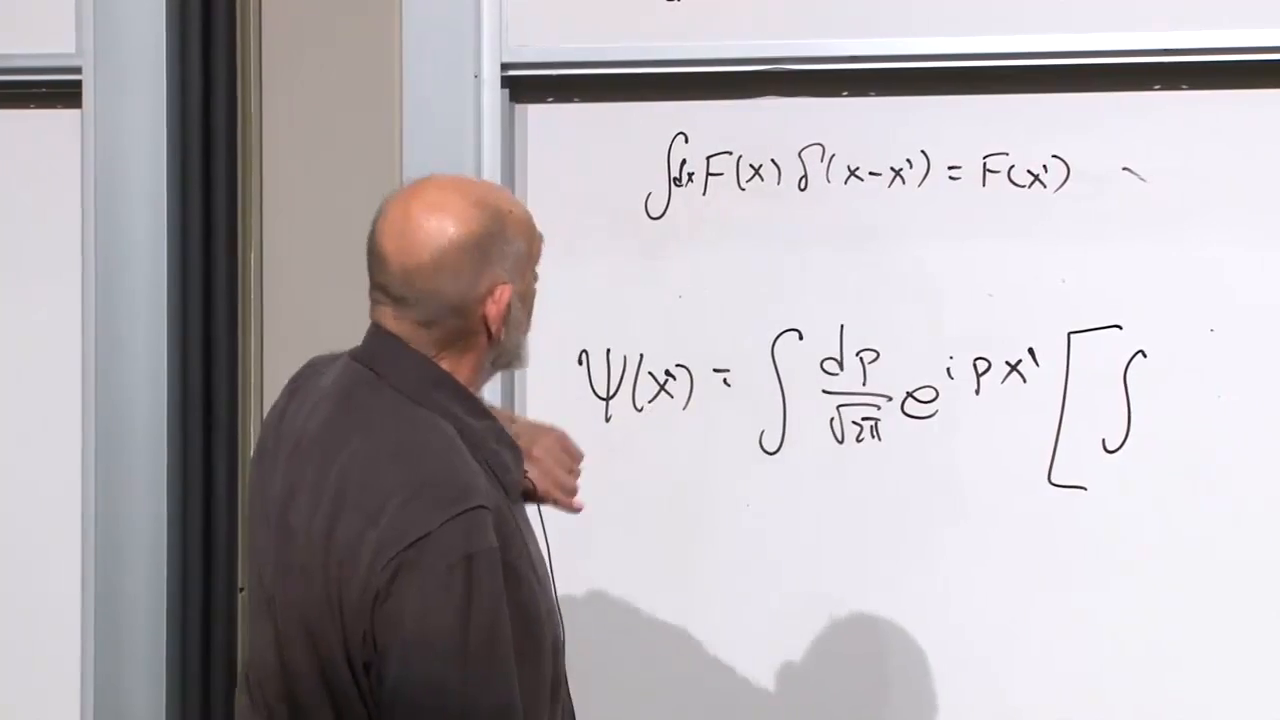
\includegraphics[width=0.88\textwidth]{lecture_09_figure_02.png}\caption{El par de Fourier simétrico: una función se descompone en ondas planas y las amplitudes de los modos se recuperan mediante la transformada inversa.}\lectureframe{00:14:35}\end{figure}

\begin{classroomqa}\audiencequestion{¿Se supone que \(\psi(x)\) y \(\widetilde{\psi}(p)\) son complejas?}\lecturerresponse{En general, sí. Una función particular puede ser real, en cuyo caso sus coeficientes de Fourier satisfacen una relación adicional de conjugación, pero las amplitudes cuánticas son naturalmente complejas y aquí no se impone ninguna condición de realidad.}\end{classroomqa}

\begin{classroomqa}\audiencequestion{¿Por qué usar los factores simétricos \(1/\sqrt{2\pi}\) en lugar de poner todo \(2\pi\) en una sola transformada?}\lecturerresponse{Cualquiera de las dos convenciones es coherente. Con la elección simétrica, las transformadas directa e inversa solo difieren en el signo del exponente. Las predicciones físicas no dependen de la convención, siempre que se cambien de manera coherente todas las normalizaciones relacionadas.}\end{classroomqa}

La relación recíproca entre \(x\) y \(p\) ya es evidente. Una función se obtiene integrando sobre la otra variable. Por ahora, esto es análisis de Fourier. Pronto, el mismo par corresponderá a la posición y el momento.

\section{La delta de Dirac como operación}

La imagen intuitiva de la función delta es la de un pico de anchura nula, altura divergente y área unidad. Esa imagen es útil, pero la definición operacional es más fiable. Para toda función de prueba adecuada \(f\),
\begin{equation}
\int_{-\infty}^{\infty}
dx\,\delta(x-x')f(x)
=f(x').
\label{eq:l9-delta-sampling}
\end{equation}
Tres reglas conocidas expresan la misma idea:
\begin{align}
f(x)\delta(x-x')
&=
f(x')\delta(x-x'),
\label{eq:l9-delta-multiplication}\\
\int_{-\infty}^{\infty}dx\,\delta(x-x')
&=1,
\label{eq:l9-delta-area}\\
\int_{-\infty}^{\infty}dx\,\delta(x-x')f(x)
&=f(x').
\end{align}
La primera regla se cumple porque la delta solo tiene soporte donde \(x=x'\). En la segunda, trasladar el pico cambia su posición, pero no su área. De esas dos reglas se deduce la tercera.

\begin{figure}[htbp]\centering
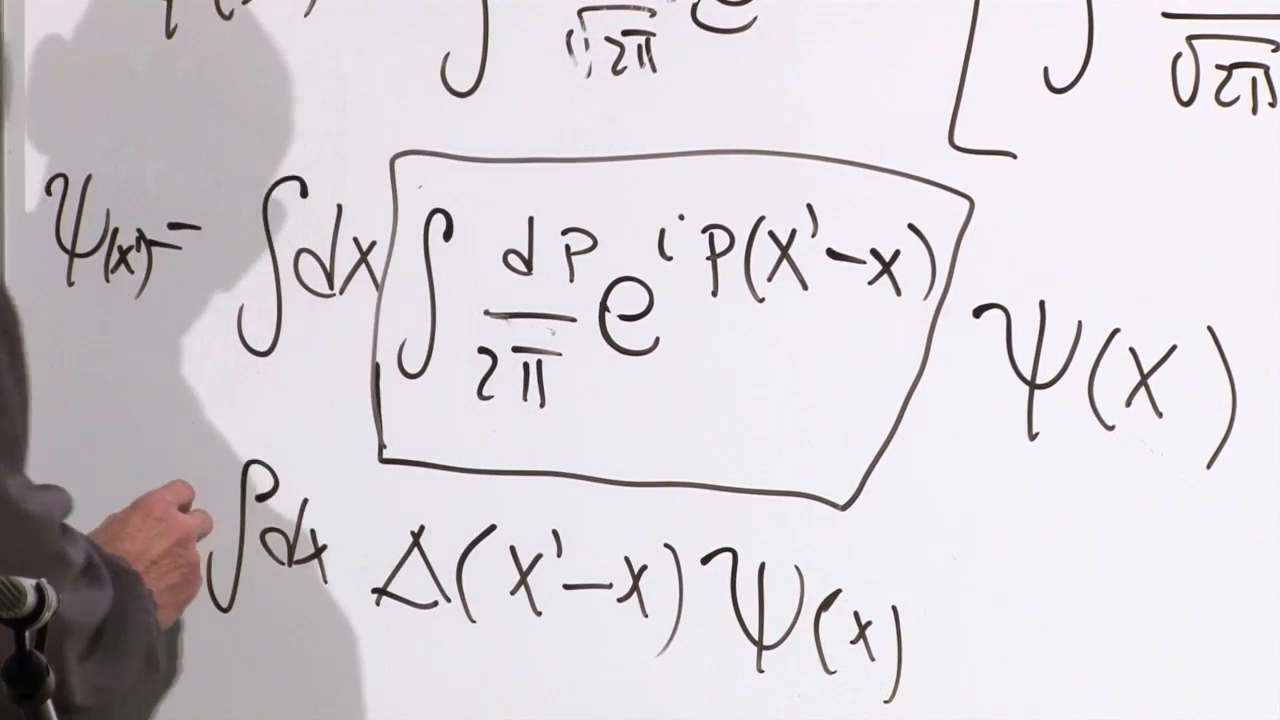
\includegraphics[width=0.88\textwidth]{lecture_09_figure_03.png}\caption{La propiedad de muestreo caracteriza la delta de Dirac por su acción sobre toda función adecuada.}\lectureframe{00:19:45}\end{figure}

\begin{classroomqa}\audiencequestion{¿Por qué se puede sacar \(f(x')\) fuera de la integral respecto de \(x\)?}\lecturerresponse{La variable de integración es \(x\). La etiqueta \(x'\) permanece fija durante esa integración, por lo que \(f(x')\) es constante respecto de \(x\). La integral de la delta que queda tiene área unidad.}\end{classroomqa}

La delta no es una función ordinaria definida punto por punto. En particular, intentar elevarla al cuadrado da lugar a un objeto más singular que la propia delta. Su significado seguro es el de una distribución: la ecuación~\eqref{eq:l9-delta-sampling} especifica cómo actúa bajo una integral.

\subsection{La representación de Fourier de la delta}

Sustituyamos la ecuación~\eqref{eq:l9-fourier-inverse} en la ecuación~\eqref{eq:l9-fourier-forward}, y cambiemos por \(x'\) el nombre del argumento del lado izquierdo:
\begin{align}
\psi(x')
&=
\int\frac{dp}{\sqrt{2\pi}}\,
e^{ipx'}
\left[
\int\frac{dx}{\sqrt{2\pi}}\,
\psi(x)e^{-ipx}
\right] \notag\\
&=
\int dx
\left[
\int\frac{dp}{2\pi}
e^{ip(x'-x)}
\right]\psi(x).
\label{eq:l9-fourier-composition}
\end{align}
La expresión entre corchetes debe reproducir \(\psi(x')\) para toda \(\psi\) adecuada. Al compararla con la acción definitoria de la delta, se obtiene
\begin{equation}
\boxed{
\int_{-\infty}^{\infty}
\frac{dp}{2\pi}\,
e^{ip(x'-x)}
=\delta(x'-x)
}.
\label{eq:l9-delta-fourier-x}
\end{equation}

\begin{figure}[htbp]\centering
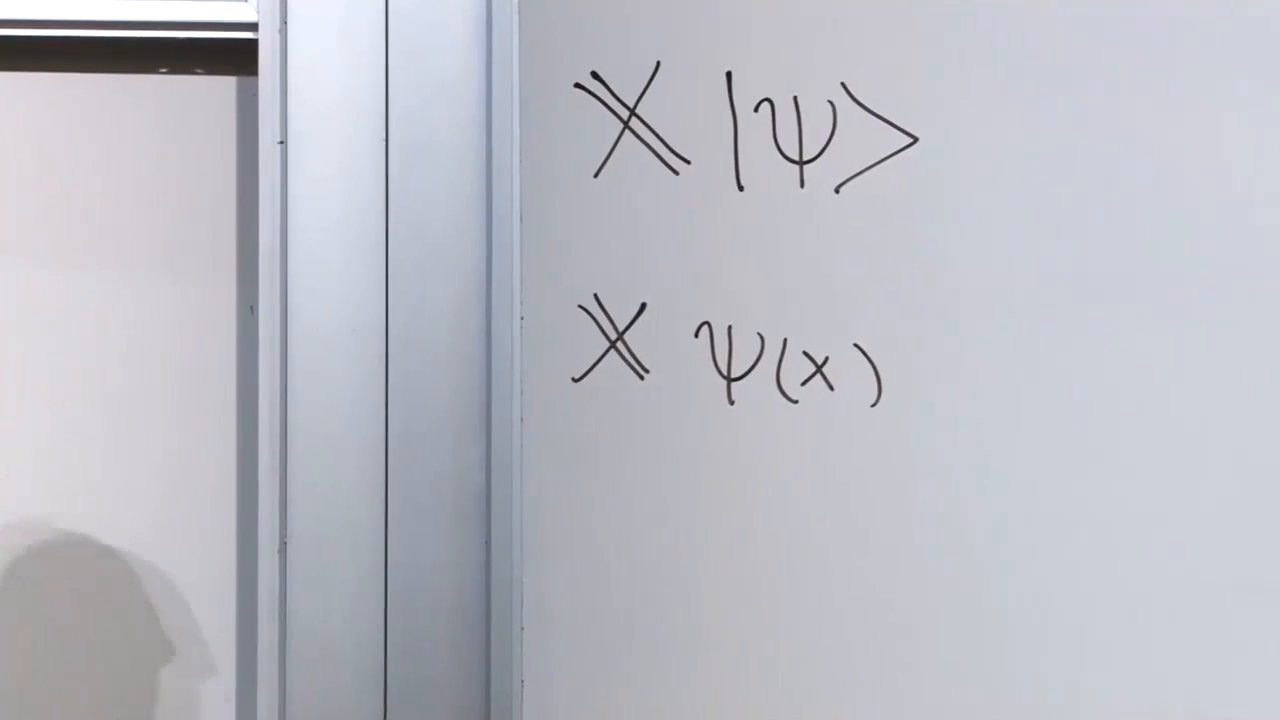
\includegraphics[width=0.88\textwidth]{lecture_09_figure_04.png}\caption{El núcleo de Fourier queda aislado al componer las dos transformadas y se identifica como una delta de Dirac por su acción de muestreo.}\lectureframe{00:26:23}\end{figure}

Al intercambiar los nombres de las variables recíprocas, se obtiene la identidad análoga
\begin{equation}
\boxed{
\int_{-\infty}^{\infty}
\frac{dx}{2\pi}\,
e^{ix(p-p')}
=\delta(p-p')
}.
\label{eq:l9-delta-fourier-p}
\end{equation}
Así, la función delta es una superposición continua de ondas planas.

\begin{classroomqa}\audiencequestion{El exponente se escribió una vez como \(x'-x\) y en otro lugar como \(x-x'\). ¿Cambia el resultado al cambiar el signo?}\lecturerresponse{No. La delta es par: \(\delta(u)=\delta(-u)\). Por tanto, invertir el signo de la diferencia deja inalterada la distribución final. El exponente intermedio pasa a ser su conjugado complejo, pero el núcleo integrado es la misma delta.}\end{classroomqa}

En estas manipulaciones se omite una salvedad sobre la convergencia. Las integrales oscilatorias son distribuciones, no integrales ordinarias absolutamente convergentes, y hay que tener cuidado al cambiar el orden de integración. Un intervalo periódico finito proporciona un regulador limpio: primero se usan modos de Fourier discretos y la ortogonalidad de Kronecker; después se hace crecer el intervalo sin límite. Las identidades continuas anteriores son el límite resultante.

\section{Una partícula en una recta}

En la mecánica clásica, un punto del espacio de fases especifica el estado:
\begin{equation}
(x,p).
\end{equation}
La mecánica cuántica empieza con una pregunta distinta: ¿qué base ortonormal define el espacio de estados? Para cada posición real \(x\), introduzcamos un ket propio generalizado \(\ket{x}\). Un estado general puede desarrollarse como
\begin{equation}
\ket{\Psi}
=
\int_{-\infty}^{\infty}
dx\,\psi(x)\ket{x},
\qquad
\psi(x)=\braket{x}{\Psi}.
\label{eq:l9-position-expansion}
\end{equation}

\begin{figure}[htbp]\centering
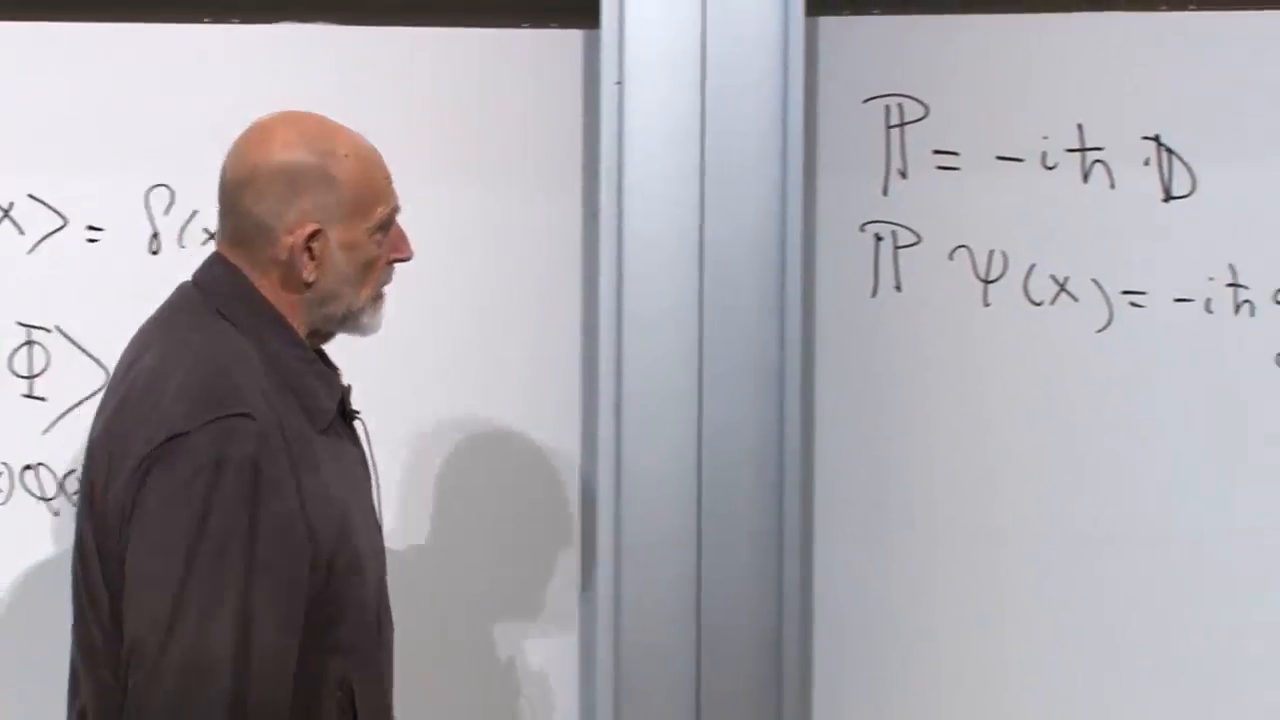
\includegraphics[width=0.88\textwidth]{lecture_09_figure_05.png}\caption{Un estado general desarrollado en la base continua de posición; el coeficiente se recupera proyectando sobre \(\ket{x}\)}\lectureframe{00:35:30}\end{figure}

La regla de Born asigna la densidad de probabilidad
\begin{equation}
\rho(x)=|\psi(x)|^2.
\end{equation}
La probabilidad de estar en un intervalo finito es
\begin{equation}
P(a<x<b)=\int_a^b|\psi(x)|^2\,dx,
\end{equation}
y un estado físico normalizado satisface
\begin{equation}
\int_{-\infty}^{\infty}|\psi(x)|^2\,dx=1.
\label{eq:l9-position-normalization}
\end{equation}
La ortogonalidad continua se expresa mediante
\begin{equation}
\braket{x'}{x}=\delta(x-x').
\label{eq:l9-position-delta}
\end{equation}
Para dos estados arbitrarios, el producto interno es
\begin{equation}
\braket{\Psi}{\Phi}
=
\int_{-\infty}^{\infty}
dx\,\psi^*(x)\phi(x).
\label{eq:l9-position-inner-product}
\end{equation}

\begin{figure}[htbp]\centering
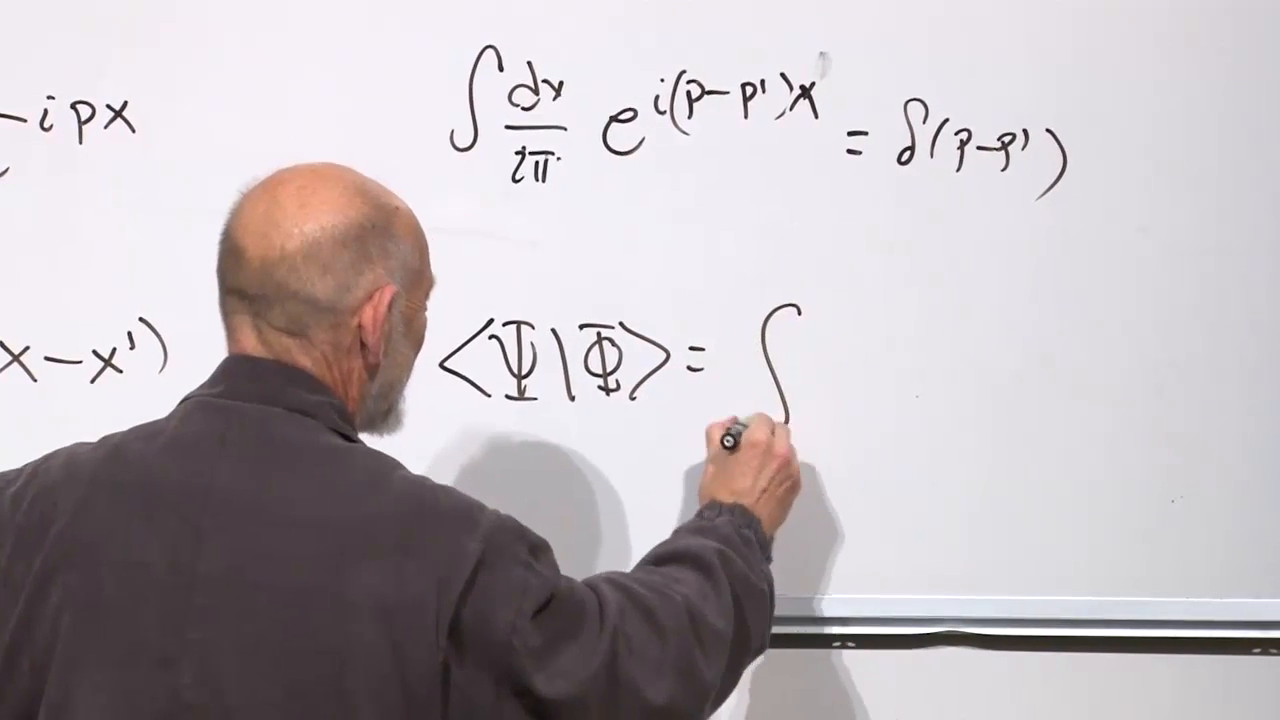
\includegraphics[width=0.88\textwidth]{lecture_09_figure_06.png}\caption{La normalización de la base continua y el producto interno de funciones de onda, expresados en la representación de posición.}\lectureframe{00:41:20}\end{figure}

\begin{classroomqa}\audiencequestion{¿Por qué basta con la posición? ¿Añadir el momento, o casi cualquier otra variable, sería redundante?}\lecturerresponse{Para una partícula en una dimensión, la función completa \(\psi(x)\) especifica el estado, así que un valor definido simultáneo de \(p\) aportaría demasiada información. El momento proporciona otra base completa, no una etiqueta adicional asociada a cada \(\ket{x}\). En más dimensiones sí se puede combinar información compatible: por ejemplo, \(X\) y \(P_y\) conmutan y pueden etiquetar una base conjunta. La restricción se refiere a pares que no conmutan, no al mero número de símbolos.}\end{classroomqa}

\begin{classroomqa}\audiencequestion{¿Puede el momento proporcionar también una base completa y desarrollarse mediante la posición?}\lecturerresponse{Sí. La base de momento es completa, y sus coeficientes están relacionados con los coeficientes de posición mediante una transformada de Fourier. Esa relación es la construcción central de esta lección.}\end{classroomqa}

\section{La posición en la representación de posición}

Un operador abstracto actúa sobre vectores de estado. Una vez elegida una base, esa misma acción se convierte en una operación concreta sobre funciones de onda. En la representación de posición, el operador de posición \(X\) actúa mediante multiplicación:
\begin{equation}
(X\psi)(x)=x\psi(x).
\label{eq:l9-position-operator}
\end{equation}

El estado localizado en \(x_0\) se representa mediante la función de onda generalizada \(\delta(x-x_0)\). Al aplicar \(X\), se obtiene
\begin{align}
X\delta(x-x_0)
&=
x\delta(x-x_0) \notag\\
&=
x_0\delta(x-x_0),
\label{eq:l9-position-eigenfunction}
\end{align}
donde se ha usado la ecuación~\eqref{eq:l9-delta-multiplication}. Así, \(\delta(x-x_0)\) es una autofunción de \(X\) con autovalor \(x_0\).

\begin{figure}[htbp]\centering
\includegraphics[width=0.88\textwidth]{lecture_09_figure_07.png}\caption{La multiplicación por \(x\) convierte el estado localizado por la delta en \(x_0\) veces el propio estado, lo que demuestra que es una autofunción de posición.}\lectureframe{00:45:50}\end{figure}

Ni \(\ket{x_0}\) ni su representante mediante la función delta están normalizados a uno en el sentido habitual de las funciones de cuadrado integrable. Están normalizados a una delta. Los estados físicos localizados son paquetes de ondas finitos, mientras que los estados propios exactos sirven como vectores de una base generalizada.

\section{Funciones propias del momento}

En la lección anterior vimos que la derivación es antihermítica y que la multiplicación por \(-i\) la hace hermítica. Al restituir las unidades, definimos
\begin{equation}
P=-i\hbar\frac{d}{dx},
\qquad
(P\psi)(x)
=
-i\hbar\frac{d\psi}{dx}.
\label{eq:l9-momentum-operator}
\end{equation}
Este es un observable legítimo en un dominio adecuado. Comprobaremos su identificación con el momento físico examinando su espectro, su longitud de onda y su papel en la dinámica.

Para un autovalor de momento \(p\), resolvamos
\begin{equation}
P\psi_p=p\psi_p,
\end{equation}
o bien
\begin{equation}
-i\hbar\frac{d\psi_p}{dx}=p\psi_p.
\end{equation}
La solución es
\begin{equation}
\psi_p(x)=A e^{ipx/\hbar}.
\label{eq:l9-momentum-eigenfunction}
\end{equation}

\begin{figure}[htbp]\centering
\includegraphics[width=0.88\textwidth]{lecture_09_figure_08.png}\caption{La representación en el espacio de posiciones de un estado de momento definido es una onda plana \(e^{ipx/\hbar}\)}\lectureframe{00:51:45}\end{figure}

La longitud de onda \(\lambda\) es el desplazamiento que adelanta la fase en \(2\pi\):
\begin{equation}
\frac{p\lambda}{\hbar}=2\pi,
\qquad
\lambda=\frac{2\pi\hbar}{p}.
\label{eq:l9-de-broglie}
\end{equation}
Por tanto, a mayor momento, menor longitud de onda.

La normalización a una delta fija la constante:
\begin{equation}
\psi_p(x)
=
\frac{1}{\sqrt{2\pi\hbar}}e^{ipx/\hbar}.
\label{eq:l9-normalized-momentum-eigenfunction}
\end{equation}
En efecto,
\begin{align}
\braket{p'}{p}
&=
\int_{-\infty}^{\infty}
dx\,
\psi_{p'}^*(x)\psi_p(x) \notag\\
&=
\int_{-\infty}^{\infty}
\frac{dx}{2\pi\hbar}
e^{i(p-p')x/\hbar} \notag\\
&=
\delta(p-p').
\label{eq:l9-momentum-normalization}
\end{align}
Tras elegir unidades en las que \(\hbar=1\), estas fórmulas quedan
\begin{equation}
\psi_p(x)=\frac{1}{\sqrt{2\pi}}e^{ipx},
\qquad
\int\frac{dx}{2\pi}e^{i(p-p')x}
=\delta(p-p').
\end{equation}

\begin{classroomqa}\audiencequestion{¿Cómo puede declararse nula la integral oscilatoria para \(p\neq p'\) si no converge en el sentido ordinario?}\lecturerresponse{La lección recurre a un atajo controlado. Se coloca el sistema en un intervalo periódico finito. Entonces los momentos permitidos forman un conjunto discreto, las exponenciales son ortogonales en el sentido ordinario y todas las normalizaciones son finitas. Solo después de ese cálculo se hace infinito el intervalo, con lo que la delta de Kronecker se convierte en una delta de Dirac.}\end{classroomqa}

\begin{classroomqa}\audiencequestion{¿Afecta el mismo problema de convergencia a la derivación de la función delta mediante la transformada de Fourier?}\lecturerresponse{Sí. Por la misma razón, allí el intercambio de integrales era formal. La derivación en una caja finita o el lenguaje de las distribuciones aporta el rigor omitido. El atajo es aceptable porque el cálculo regulado tiene el límite continuo indicado.}\end{classroomqa}

\section{La representación de momento}

No hay que confundir dos objetos. La función \(\psi_p(x)\) de la ecuación~\eqref{eq:l9-normalized-momentum-eigenfunction} es la representación en el espacio de posiciones del estado propio particular \(\ket{p}\). En cambio, la función de onda en el espacio de momentos de un estado arbitrario \(\ket{\Psi}\) es
\begin{equation}
\widetilde{\psi}(p)=\braket{p}{\Psi}.
\label{eq:l9-momentum-wavefunction}
\end{equation}
Sustituyamos las funciones de onda en el espacio de posiciones de \(\bra{p}\) y \(\ket{\Psi}\):
\begin{align}
\widetilde{\psi}(p)
&=
\int_{-\infty}^{\infty}
dx\,
\braket{p}{x}\braket{x}{\Psi} \notag\\
&=
\int_{-\infty}^{\infty}
\frac{dx}{\sqrt{2\pi\hbar}}\,
e^{-ipx/\hbar}\psi(x).
\label{eq:l9-position-to-momentum}
\end{align}
Esta es precisamente la transformada de Fourier. A la inversa,
\begin{equation}
\psi(x)
=
\int_{-\infty}^{\infty}
\frac{dp}{\sqrt{2\pi\hbar}}\,
\widetilde{\psi}(p)e^{ipx/\hbar}.
\label{eq:l9-momentum-to-position}
\end{equation}

\begin{figure}[htbp]\centering
\includegraphics[width=0.88\textwidth]{lecture_09_figure_09.png}\caption{La proyección sobre \(\ket{p}\) convierte la función de onda en el espacio de posiciones en su transformada de Fourier, \(\widetilde{\psi}(p)\).}\lectureframe{01:05:50}\end{figure}

La densidad de probabilidad de medir el momento \(p\) es
\begin{equation}
\widetilde{\rho}(p)
=
|\widetilde{\psi}(p)|^2,
\qquad
\int_{-\infty}^{\infty}
|\widetilde{\psi}(p)|^2\,dp=1.
\end{equation}
Así pues, una sola función de onda en el espacio de posiciones contiene información suficiente para predecir tanto las mediciones de posición como las de momento. Para obtener las probabilidades del momento, se calcula la transformada de Fourier de \(\psi(x)\) y se eleva el módulo del resultado al cuadrado.

En la representación de momento, los papeles se invierten:
\begin{equation}
(P\widetilde{\psi})(p)
=
p\widetilde{\psi}(p),
\qquad
(X\widetilde{\psi})(p)
=
i\hbar\frac{d\widetilde{\psi}}{dp}.
\label{eq:l9-operators-in-p}
\end{equation}
La diferencia de signo respecto de \(P=-i\hbar\,d/dx\) se debe a que los signos del par de Fourier son opuestos.

\begin{classroomqa}\audiencequestion{¿Es el tiempo el operador conjugado de la energía, del mismo modo que la posición es conjugada del momento?}\lecturerresponse{Por lo general, el tiempo se trata como el parámetro externo que etiqueta la evolución del estado, no como un operador autoadjunto universal en el espacio de Hilbert del sistema. Un reloj físico sí tiene lecturas observables, y mejorar su resolución temporal tiene consecuencias energéticas, pero la relación tiempo-energía requiere más cuidado que el par posición-momento y no se desarrollará aquí.}\end{classroomqa}

\begin{classroomqa}\audiencequestion{¿Qué otros pares conjugados hay?}\lecturerresponse{El ángulo y el momento angular correspondiente constituyen un ejemplo importante, con salvedades globales porque el ángulo es periódico. En teoría de campos, un campo y su momento canónico son conjugados. La temperatura y la presión son variables termodinámicas, no un par cuántico canónico. El principio general lo proporcionan las variables canónicas y sus conmutadores, no cualquier par arbitrario de magnitudes medibles.}\end{classroomqa}

\begin{classroomqa}\audiencequestion{En la teoría discreta, los operadores actuaban sobre kets y las funciones de onda se limitaban a enumerar coeficientes. ¿Ha cambiado eso en la teoría continua?}\lecturerresponse{No. Una función de onda es la columna de coordenadas de un ket abstracto en una base elegida. Una matriz que actúa sobre una columna finita y un operador diferencial o integral que actúa sobre una función son dos representaciones concretas de la misma operación abstracta. La etiqueta continua cambia la notación, no la lógica.}\end{classroomqa}

\subsection{La incertidumbre como hecho de Fourier}

Un estado de momento definido está completamente deslocalizado:
\begin{equation}
|\psi_p(x)|^2=\text{constant}.
\end{equation}
Su momento está definido con precisión, pero su posición se distribuye uniformemente a lo largo de la recta. En general, los dos miembros de un par de Fourier no pueden ser ambos estrechos. Concentrar \(\widetilde{\psi}(p)\) en un intervalo pequeño de momentos obliga a \(\psi(x)\) a extenderse por una región amplia, y localizar \(\psi(x)\) requiere un intervalo amplio de momentos.

La lección todavía no deduce la desigualdad cuantitativa
\begin{equation}
\Delta X\,\Delta P\geq\frac{\hbar}{2}.
\end{equation}
Por ahora, el punto es estructural: el principio de incertidumbre ya está codificado en la geometría recíproca de las transformadas de Fourier. Este es el análogo continuo del cambio entre bases de espín incompatibles.

\section{El hamiltoniano genera la evolución temporal}

El hamiltoniano \(H\) es hermítico, representa la energía y genera la evolución temporal unitaria. La ecuación de Schr\"odinger dependiente del tiempo es
\begin{equation}
i\hbar\frac{d}{dt}\ket{\Psi(t)}
=
H\ket{\Psi(t)}.
\label{eq:l9-abstract-schrodinger}
\end{equation}
En la representación de posición,
\begin{equation}
i\hbar\frac{\partial\psi(x,t)}{\partial t}
=
H\psi(x,t),
\label{eq:l9-position-schrodinger}
\end{equation}
donde el lado derecho representa la acción sobre la función del hamiltoniano en la representación de posición elegida.

\subsection{Un hamiltoniano lineal deliberadamente sencillo}

Tomemos
\begin{equation}
H=cP.
\label{eq:l9-linear-hamiltonian}
\end{equation}
Este no es el hamiltoniano habitual de una partícula libre no relativista. Se elige porque permite ver directamente cada paso.

\begin{figure}[htbp]\centering
\includegraphics[width=0.88\textwidth]{lecture_09_figure_10.png}\caption{La ecuación de Schr\"odinger y el hamiltoniano lineal \(H=cP\), elegido como el ejemplo más sencillo de evolución de una partícula.}\lectureframe{01:17:45}\end{figure}

Usando \(P=-i\hbar\,\partial_x\),
\begin{align}
i\hbar\frac{\partial\psi}{\partial t}
&=
c\left(-i\hbar\frac{\partial}{\partial x}\right)\psi, \notag\\
\frac{\partial\psi}{\partial t}
&=
-c\frac{\partial\psi}{\partial x},
\end{align}
o bien
\begin{equation}
\frac{\partial\psi}{\partial t}
+c\frac{\partial\psi}{\partial x}=0.
\label{eq:l9-transport-equation}
\end{equation}

\begin{figure}[htbp]\centering
\includegraphics[width=0.88\textwidth]{lecture_09_figure_11.png}\caption{El hamiltoniano lineal reduce la ecuación de Schr\"odinger a la ecuación de transporte de primer orden.}\lectureframe{01:20:05}\end{figure}

La solución general es
\begin{equation}
\psi(x,t)=f(x-ct),
\label{eq:l9-rigid-translation}
\end{equation}
para cualquier perfil inicial normalizable \(f\). En el instante \(t=0\), el perfil es \(f(x)\). En instantes posteriores, cada rasgo se ha desplazado hacia la derecha una distancia \(ct\). La función de onda compleja, sus partes real e imaginaria y su densidad de probabilidad conservan todas su forma:
\begin{equation}
|\psi(x,t)|^2=|f(x-ct)|^2.
\end{equation}
En consecuencia,
\begin{equation}
\expect{X}_t=\expect{X}_0+ct.
\end{equation}

Se eligió el símbolo \(c\) para evocar la velocidad de la luz. El modelo se parece a una excitación quiral, sin masa y unidimensional: todas las componentes permitidas se mueven en un mismo sentido y con la misma velocidad. No es una teoría completa del fotón. Los fonones unidimensionales de baja energía con una velocidad del sonido fija ofrecen otra analogía. Como \(E=cp\), permitir ambos signos de \(p\) también permite energías negativas, otra señal de que se trata de un modelo didáctico deliberadamente restringido.

\begin{classroomqa}\audiencequestion{¿Describiría \(H=cP\) cualquier partícula libre si se sustituyera \(c\) por la velocidad de esa partícula?}\lecturerresponse{No. Un coeficiente fijo en \(H=cP\) indica que todas las componentes de momento tienen la misma velocidad. Para una partícula no relativista, la velocidad es \(p/m\), por lo que depende del momento. Escribir \(vP\) con \(v=p/m\) deja de ser lineal en \(P\) y apunta a un hamiltoniano cuadrático.}\end{classroomqa}

\begin{classroomqa}\audiencequestion{¿No debería la función de onda de un electrón libre ordinario trasladarse simplemente sin deformarse?}\lecturerresponse{Solo una relación de dispersión muy particular produce una traslación rígida de cualquier perfil. Un paquete de ondas de un electrón libre ordinario contiene muchas componentes de momento cuyas fases evolucionan a ritmos distintos. Su centro se desplaza, pero, en general, su forma se dispersa.}\end{classroomqa}

\subsection{Comparación clásica}

Para el hamiltoniano clásico \(H=cp\), las ecuaciones de Hamilton dan
\begin{equation}
\dot{x}=\frac{\partial H}{\partial p}=c,
\qquad
\dot{p}=-\frac{\partial H}{\partial x}=0.
\label{eq:l9-linear-hamilton-equations}
\end{equation}

\begin{figure}[htbp]\centering
\includegraphics[width=0.88\textwidth]{lecture_09_figure_12.png}\caption{Ecuaciones de Hamilton para \(H=cp\): velocidad constante hacia la derecha y momento conservado.}\lectureframe{01:25:20}\end{figure}

La distribución de probabilidad cuántica y su valor esperado obedecen el mismo movimiento elemental. Esta concordancia recuerda, por primera vez de forma concreta, que la evolución cuántica construida a partir de un hamiltoniano clásico debe reproducir las ecuaciones clásicas en el sentido adecuado.

\section{La partícula libre no relativista}

Para una partícula ordinaria de masa \(m\) sin fuerza, la energía cinética clásica es
\begin{equation}
H=\frac{p^2}{2m}.
\end{equation}
La forma cuadrática trata \(p\) y \(-p\) simétricamente, de modo que las partículas que se mueven a izquierda o derecha tienen la misma energía positiva. La cuantización sustituye \(p\) por el operador \(P\):
\begin{equation}
H=\frac{P^2}{2m}.
\label{eq:l9-free-hamiltonian}
\end{equation}
Sustituyamos \(P=-i\hbar\,\partial_x\) en la ecuación de Schr\"odinger:
\begin{align}
i\hbar\frac{\partial\psi}{\partial t}
&=
\frac{1}{2m}
\left(-i\hbar\frac{\partial}{\partial x}\right)^2
\psi \notag\\
&=
-\frac{\hbar^2}{2m}
\frac{\partial^2\psi}{\partial x^2}.
\label{eq:l9-free-schrodinger}
\end{align}

\begin{figure}[htbp]\centering
\includegraphics[width=0.88\textwidth]{lecture_09_figure_13.png}\caption{La ecuación de Schr\"odinger para una partícula libre, obtenida a partir de \(H=P^2/(2m)\) y \(P=-i\hbar\,\partial_x\).}\lectureframe{01:33:50}\end{figure}

Una componente de onda plana con momento \(p\) tiene energía
\begin{equation}
E(p)=\frac{p^2}{2m}.
\end{equation}
A diferencia del caso lineal \(E=cp\), la pendiente de esta relación de dispersión depende de \(p\):
\begin{equation}
v_{\mathrm{group}}
=
\frac{dE}{dp}
=
\frac{p}{m}.
\end{equation}
Por tanto, las distintas componentes de momento de un paquete localizado viajan con distintas velocidades de grupo. Sus fases relativas cambian, las componentes se separan y el paquete se dispersa. La diferencia decisiva es que \(H=cP\) transporta rígidamente cualquier perfil, mientras que \(H=P^2/(2m)\) produce el movimiento dispersivo de una partícula libre.

\section{Qué se ha establecido}

La digresión matemática no estaba separada de la física. Las ondas planas y la delta de Dirac proporcionaron las herramientas para construir una base continua. El operador de posición actúa mediante multiplicación, el operador de momento actúa mediante derivación y los estados propios del momento son ondas planas. La proyección de un estado arbitrario sobre esos estados propios produce la transformada de Fourier de su función de onda en el espacio de posiciones. Por tanto, posición y momento son representaciones alternativas de un mismo estado, y su incertidumbre es la conocida relación recíproca entre las anchuras de un par de Fourier.

Este mismo formalismo de representaciones convierte después un hamiltoniano en una ecuación diferencial. Una función lineal del momento produce una traslación rígida; la energía cinética cuadrática produce la ecuación de Schr\"odinger para una partícula libre y la dispersión. El curso ha pasado de los fundamentos de la medición a la mecánica del movimiento sin cambiar su lenguaje central: estados, bases, observables hermíticos, amplitudes y evolución unitaria.
